\subsection{Blur}

\Fig~\ref{fig:acc_bl_wu} presents the results obtained using altered data with blur for both the BNN and standard NN. \Fig~\ref{fig:bl_acc_wu_bnn} shows the accuracy trend of the BNN, while \Fig~\ref{fig:blur_ann} the trend for the standard NN. The behavior is again the same, the curve has the shape of low-pass filter. The accuracy of standard NN starts at a level greater than the on of BNN, showing to be more robust. Furthermore, the standard NN degrades less than the BNN.

\begin{figure}[h]
	\centering
	\begin{subfigure}{.5\textwidth}
		\centering
		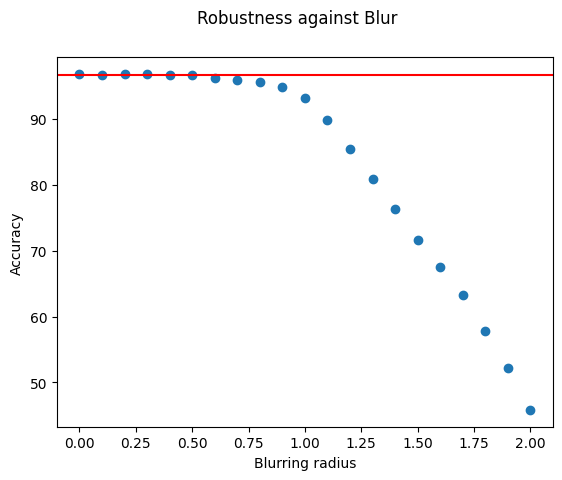
\includegraphics[width=0.8\linewidth]{ImageFiles/EvalBNN/BL/WU/acc}
		\caption{BNN}
		\label{fig:bl_acc_wu_bnn}
	\end{subfigure}%
	\begin{subfigure}{.5\textwidth}
		\centering
		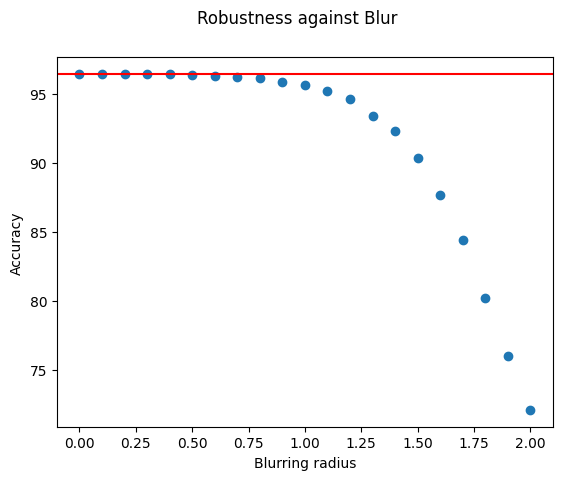
\includegraphics[width=0.8\linewidth]{ImageFiles/EvalANN/blur_ann}
		\caption{Standard NN}
		\label{fig:blur_ann}
	\end{subfigure}
	\caption{Accuracy trend for blur alteration}
	\label{fig:acc_bl_wu}
\end{figure}

When computing robustness, the results are $0.9331$ for the BNN and $0.9601$ for the standard NN, which demonstrates to be more robust than the BNN with this setting.

\Fig~\ref{fig:bl_uncertainty} shows the trend of uncertainty estimated by the BNN. In particular, \Fig~\ref{fig:bl_aleatoric} illustrates the aleatoric uncertainty trend, while \Fig~\ref{fig:bl_epistemic} presents the epistemic uncertainty.

It is worth noting that in this case the uncertainty values have a different shape. The aleatoric uncertainty has a more outlined shape, similar to a ramp that starts to increase for a blurring radius around $0.50$, following a linear trajectory. The epistemic uncertainty increases for a blurring radius around $0.75$ more like an exponential function.

\begin{figure}[h]
	\centering
	\begin{subfigure}{.5\textwidth}
		\centering
		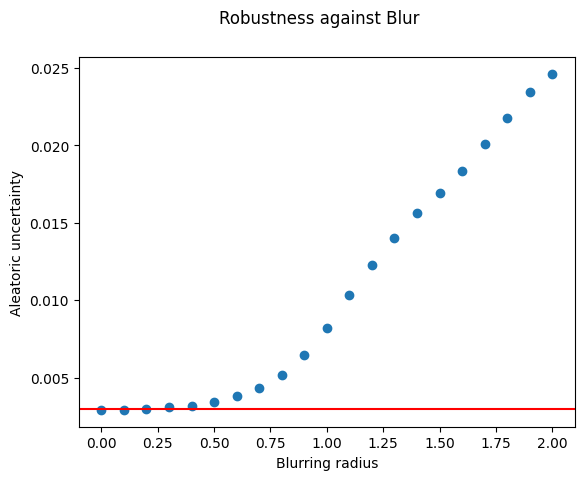
\includegraphics[width=0.8\linewidth]{ImageFiles/EvalBNN/BL/aleatoric}
		\caption{Aleatoric uncertainty}
		\label{fig:bl_aleatoric}
	\end{subfigure}%
	\begin{subfigure}{.5\textwidth}
		\centering
		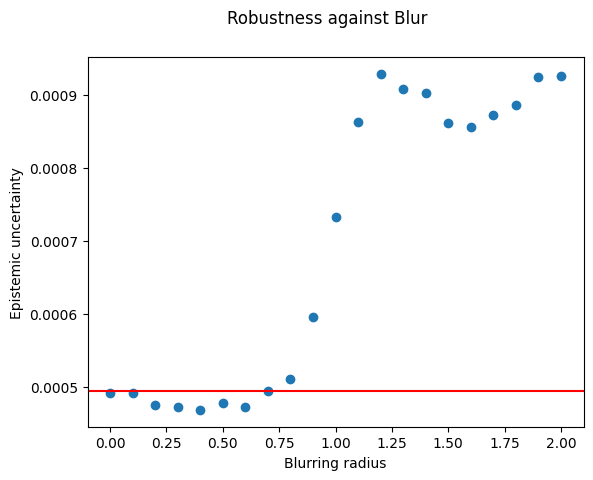
\includegraphics[width=0.8\linewidth]{ImageFiles/EvalBNN/BL/epistemic}
		\caption{Epistemic uncertainty}
		\label{fig:bl_epistemic}
	\end{subfigure}
	\caption{Uncertainty trend for blur alteration}
	\label{fig:bl_uncertainty}
\end{figure}

The next analysis will focus on evaluating whether the estimated uncertainty utilization contributes to performance improvement.

\vspace{0.3cm}
\textbf{Classification using aleatoric uncertainty}
\vspace{0.1cm}

In \Fig~\ref{fig:bl_au}, the results of the BNN evaluation on the dataset altered with blur filter are illustrated, where aleatoric uncertainty is utilized as a metric to implement the ``I don't know behavior". \Fig~\ref{fig:bl_au_acc} shows that there is an improvement in the accuracy, which starts to decrease for blurring radius around $1.10$, following the same trajectory.

However, \Fig~\ref{fig:bl_au_unkn} shows that there is a significant increase in the unknown ratio. This is reflected  by the effectiveness, as seen in \Fig~\ref{fig:bl_au_eff}, which starts to decrease around $0.50$. This can be identified as the blurring radius limit concerning robustness.

\begin{figure}[h]
	\centering
	\begin{subfigure}{.33\textwidth}
		\centering
		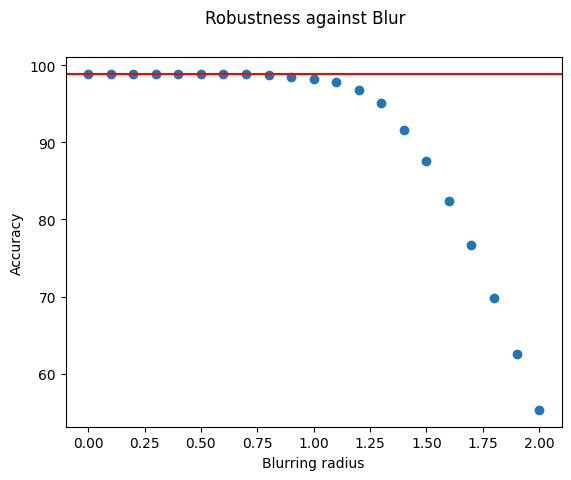
\includegraphics[width=0.9\linewidth]{ImageFiles/EvalBNN/BL/AU/acc}
		\caption{Accuracy using aleatoric \\ uncertainty}
		\label{fig:bl_au_acc}
	\end{subfigure}%
	\begin{subfigure}{.33\textwidth}
		\centering
		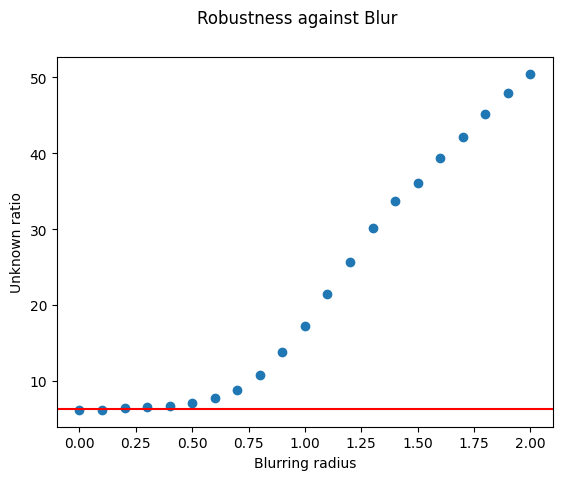
\includegraphics[width=0.9\linewidth]{ImageFiles/EvalBNN/BL/AU/unkn}
		\caption{Unknown ratio using aleatoric uncertainty}
		\label{fig:bl_au_unkn}
	\end{subfigure}%
	\begin{subfigure}{.33\textwidth}
		\centering
		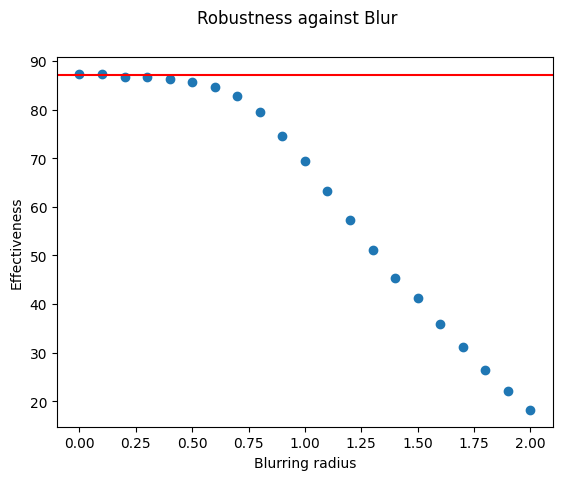
\includegraphics[width=0.9\linewidth]{ImageFiles/EvalBNN/BL/AU/eff}
		\caption{Effectiveness using aleatoric uncertainty}
		\label{fig:bl_au_eff}
	\end{subfigure}
	\caption{Robustness graph for blur when aleatoric uncertainty is employed in the classification}
	\label{fig:bl_au}
\end{figure}

\Tab~\ref{table:rob_bl_au} provides a summary of the robustness metrics resulting from this evaluation. It is possible to note that the robustness increased, but the presence of the unknown values penalizes the augmented robustness.

\begin{table}[h]
	\centering
	\begin{tabular}{|| l | l ||} 
		\hline
		\textbf{Parameter} & \textbf{Value} \\
		\hline
		\hline
		$rob_{Blur}$ & $0.9616$ \\
		$robInd_{Blur}$ & $0.9160$ \\
		$robAug_{Blur}$ & $0.8590$ \\	
		\hline
	\end{tabular}	
	\caption{Robustness metrics for the blur when the aleatoric uncertainty is employed}
	\label{table:rob_bl_au}
\end{table}

This analysis highlights how the network can identify situations of uncertainty, but this penalizes the unknown ratio, causing it to increase rapidly. When utilizing aleatoric uncertainty, the network remains robust until the blurring radius is lower than $0.75$, after which the effectiveness drops rapidly.

\vspace{0.3cm}
\textbf{Classification using epistemic uncertainty}
\vspace{0.1cm}

\Fig~\ref{fig:bl_eu} presents the results obtained from the evaluation using epistemic uncertainty.

The accuracy trend appears to follow the same shape. In this case, it seems to be very similar to the case without the use of uncertainty. In fact, the unknown ratio remains low, as seen in \Fig~\ref{fig:bl_eu_unkn}, without following any specific trajectory. The effectiveness trend in \Fig~\ref{fig:bl_eu_eff} reveals a better behavior than the previous case. It begins to decrease around the same blurring radius of $0.75$, but in this case, the decrease is less rapid.

\begin{figure}[h]
	\centering
	\begin{subfigure}{.33\textwidth}
		\centering
		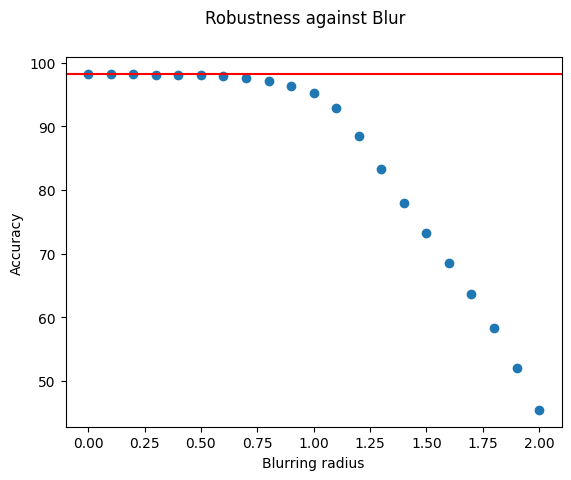
\includegraphics[width=0.9\linewidth]{ImageFiles/EvalBNN/BL/EU/acc}
		\caption{Accuracy using epistemic \\ uncertainty}
		\label{fig:bl_eu_acc}
	\end{subfigure}%
	\begin{subfigure}{.33\textwidth}
		\centering
		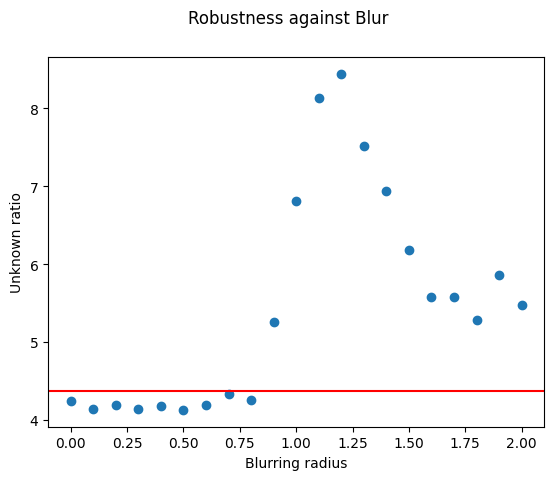
\includegraphics[width=0.9\linewidth]{ImageFiles/EvalBNN/BL/EU/unkn}
		\caption{Unknown ratio using \\ epistemic uncertainty}
		\label{fig:bl_eu_unkn}
	\end{subfigure}%
	\begin{subfigure}{.33\textwidth}
		\centering
		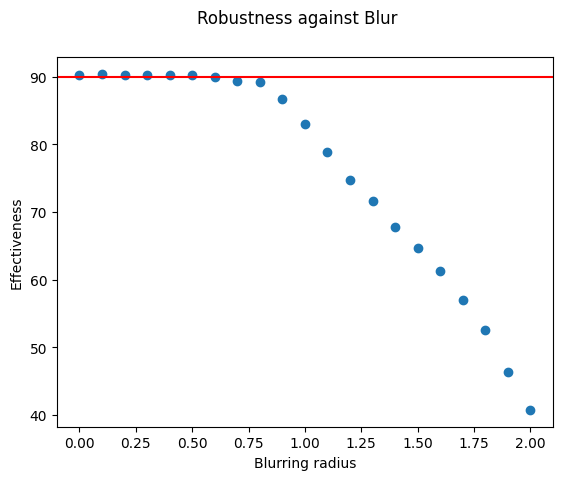
\includegraphics[width=0.9\linewidth]{ImageFiles/EvalBNN/BL/EU/eff}
		\caption{Effectiveness using \\ epistemic uncertainty}
		\label{fig:bl_eu_eff}
	\end{subfigure}
	\caption{Robustness graph for blur when epistemic uncertainty is employed in the classification}
	\label{fig:bl_eu}
\end{figure}

\Tab~\ref{table:rob_bl_eu} provides a summary of the observations made thus far. The $robAug$ has a significantly higher value than the previous case, at the cost of a lower $rob$ value.

\begin{table}[h]
	\centering
	\begin{tabular}{|| l | l ||} 
		\hline
		\textbf{Parameter} & \textbf{Value} \\
		\hline
		\hline
		$rob_{Blur}$ & $0.9339$ \\
		$robInd_{Blur}$ & $0.9937$ \\
		$robAug_{Blur}$ & $0.9246$ \\	
		\hline
	\end{tabular}	
	\caption{Robustness metrics for the blur when the epistemic uncertainty is employed}
	\label{table:rob_bl_eu}
\end{table}

In this case the epistemic uncertainty behaves better, even if it does not show any clear trend in the unknown values.

\vspace{0.3cm}
\textbf{Classification using standard deviation}
\vspace{0.1cm}

With the standard deviation, as shown in \Fig~\ref{fig:bl_vu_acc}, it possible to improve the performance in terms of accuracy. However \Fig~\ref{fig:bl_vu_unkn} shows that this improvement has strong consequences in terms of unknown ratio. In fact, as seen in \Fig~\ref{fig:bl_vu_eff}, the effectiveness starts to drop earlier than the previous cases.

\begin{figure}[h]
	\centering
	\begin{subfigure}{.33\textwidth}
		\centering
		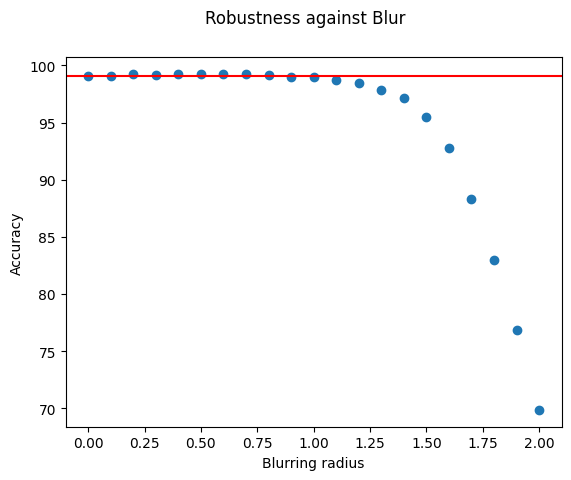
\includegraphics[width=0.9\linewidth]{ImageFiles/EvalBNN/BL/VU/acc}
		\caption{Accuracy using standard \\ deviation}
		\label{fig:bl_vu_acc}
	\end{subfigure}%
	\begin{subfigure}{.33\textwidth}
		\centering
		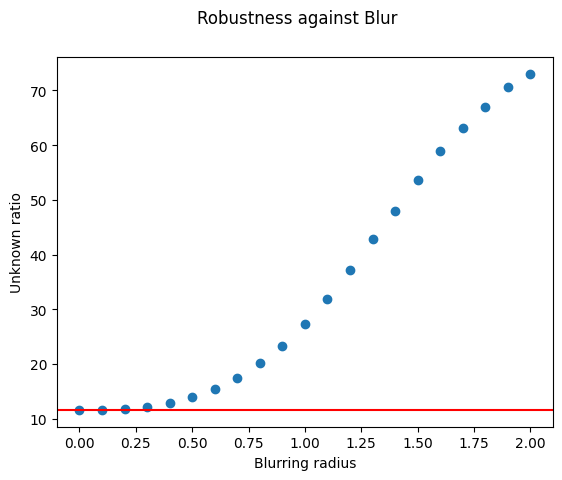
\includegraphics[width=0.9\linewidth]{ImageFiles/EvalBNN/BL/VU/unkn}
		\caption{Unknown ratio using \\ standard deviation}
		\label{fig:bl_vu_unkn}
	\end{subfigure}%
	\begin{subfigure}{.33\textwidth}
		\centering
		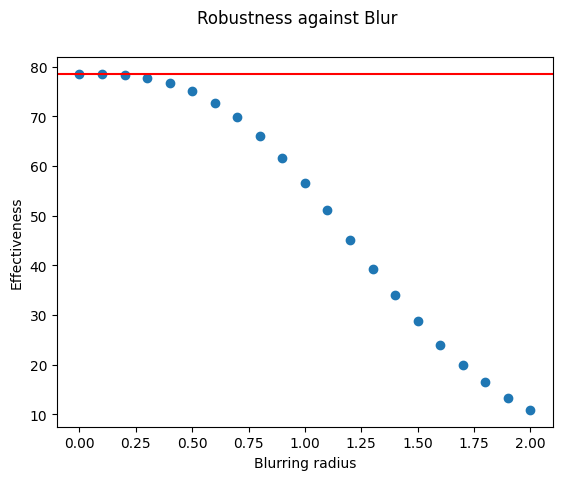
\includegraphics[width=0.9\linewidth]{ImageFiles/EvalBNN/BL/VU/eff}
		\caption{Effectiveness using standard deviation}
		\label{fig:bl_vu_eff}
	\end{subfigure}
	\caption{Robustness graph for blur when standard deviation is employed in the classification}
	\label{fig:bl_vu}
\end{figure}

\Tab~\ref{table:rob_bl_vu} provides the three robustness metrics. Although the $rob$ is higher, the other two indicators reveal a significant weakness in this setting, making it not a favorable choice in this case.

\begin{table}[h]
	\centering
	\begin{tabular}{|| l | l ||} 
		\hline
		\textbf{Parameter} & \textbf{Value} \\
		\hline
		\hline
		$rob_{Blur}$ & $0.9803$ \\
		$robInd_{Blur}$ & $0.8728$ \\
		$robAug_{Blur}$ & $0.8275$ \\	
		\hline
	\end{tabular}	
	\caption{Robustness metrics for the blur when the standard deviation is employed}
	\label{table:rob_bl_vu}
\end{table}

\vspace{0.3cm}
\textbf{Comparison}
\vspace{0.1cm}

\Tab~\ref{table:rob_bl} presents a summary of the results obtained using the different classification methods. In this case, only the aleatoric uncertainty and standard deviation achieve improved robustness in terms of accuracy. On the other hand, epistemic uncertainty serves as a better alternative in terms of effectiveness, as it maintains a good trade-off between accuracy and the unknown ratio. Therefore, in this setting, aleatoric uncertainty is preferable when the goal is to achieve high accuracy, while epistemic uncertainty is suitable for keeping a low unknown ratio. In general, it appears that the BNN struggles to successfully identify uncertain cases with blur, suggesting that this particular alteration may pose a challenge for the network.

\begin{table}[h]
	\centering
	\begin{tabular}{|| l | l | l | l ||} 
		\hline
		\textbf{Parameter} & \textbf{Aleatoric} & \textbf{Epistemic} & \textbf{Standard deviation} \\
		\hline
		\hline
		$rob_{Blur}$ & $0.9616$ & $0.9339$ & $0.9803$ \\
		$robInd_{Blur}$ & $0.9160$ & $0.9937$ & $0.8728$ \\
		$robAug_{Blur}$ & $0.8590$ & $0.9246$ & $0.8275$ \\	
		\hline
	\end{tabular}	
	\caption{Summary of the robustness metrics for the blur alteration}
	\label{table:rob_bl}
\end{table}